\chapter{Implementasi dan Pengujian}

Pada bab ini akan dijelaskan mengenai implementasi, pengujian, dan masalah yang dihadapi saat implementasi. 

\section{Implementasi}
Aplikasi dikembangkan dengan Android Studio, dengan sebuah \textit{laptop} . Aplikasi dijalankan pada tiga buah ponsel Android.

\subsection{Lingkunan Implementasi}
Berikut adalah spesifikasi \textit{laptop} dan kakas yang digunakan untuk implementasi:

\begin{enumerate}
	\item \textit{Processor} : Intel(R) Core(TM) i7-7700HQ CPU @ 2.80GHz.
	
	\item RAM : 16.0 GB (15.9 GB usable).
	
	\item Versi Android Studio : 4.1.1
	
	\item Google VR for Android : 1.190.0
\end{enumerate}

Berikut adalah spesifikasi ponsel Android yang digunakan untuk implementasi:

\begin{enumerate}
	\item Processor : Qualcomm Snapdragon 835
	
	\item Sistem Operasi : Android 9.0 (Pie)
	
	\item Sensor yang dimiliki : Accelerometer, gyroscope, magnetometer, step detector.  
\end{enumerate}

\subsection{Hasil Implementasi}
Yang dihasilkan dari implementasi ini adalah aplikasi VR untuk berlari. Aplikasi dapat diperoleh di Google Play Store dan dapat di-\textit{install} pada gawai dengan sistem operasi Android. 

\subsection{Tampilan Ketika Aplikasi Pertama Kali Dibuka}
Ketika pengguna membuka aplikasi pertama kali, akan ada judul aplikasi , dua \textit{text box}, dan satu buah tombol bertuliskan \textit{"Start Running"}. Gambar \ref{fig:main-page} menggambarkan tampilan aplikasi dan Gambar \ref{fig:user-main-page} mengilustrasikan \textit{state} pengguna saat itu.

\begin{figure}
\minipage{0.5\textwidth}
  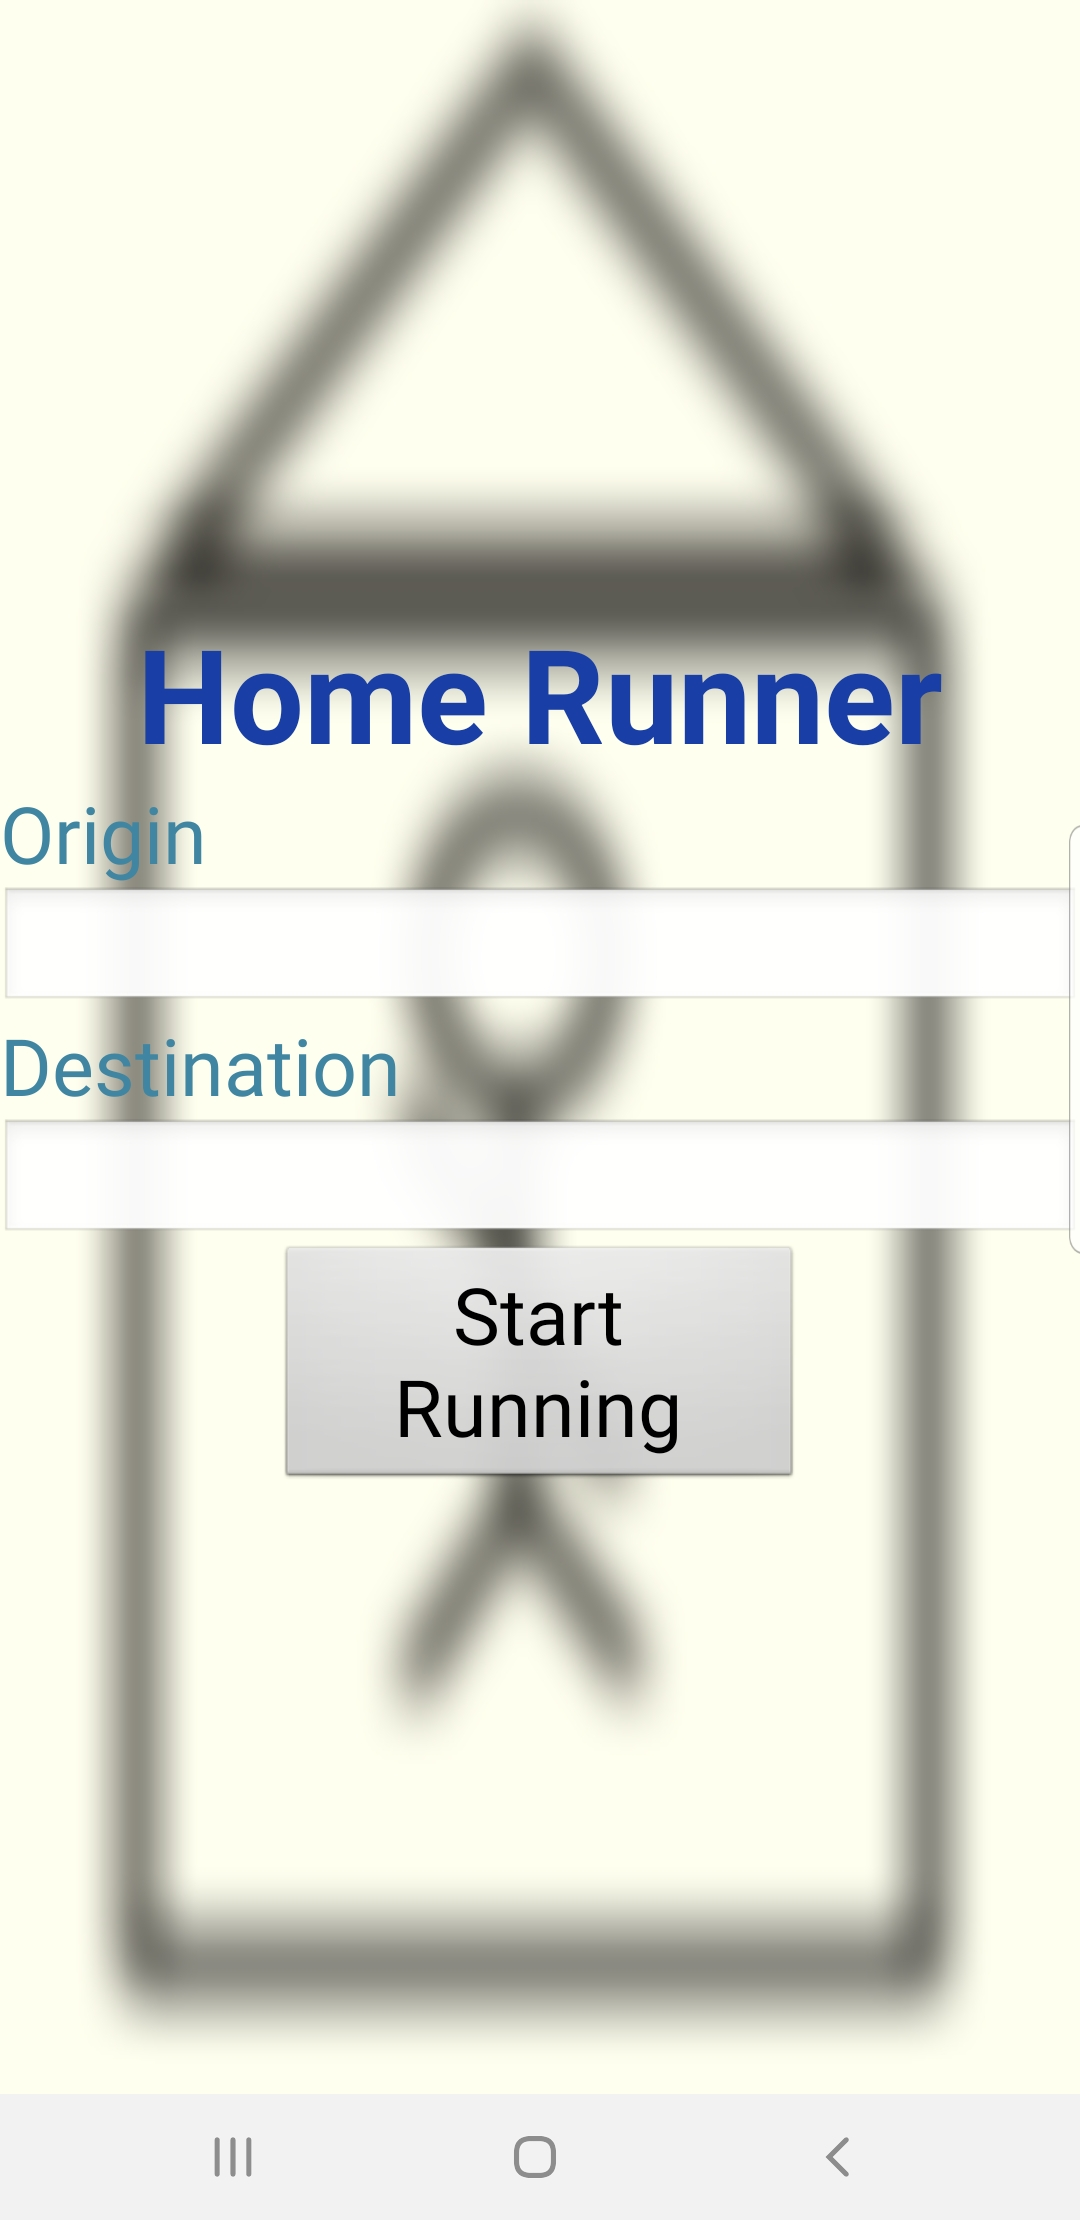
\includegraphics[scale=0.15]{Gambar/main-page.png}
  \caption{\textit{Activity} utama aplikasi}
  \label{fig:main-page}
\endminipage\hfill
\minipage{0.5\textwidth}
  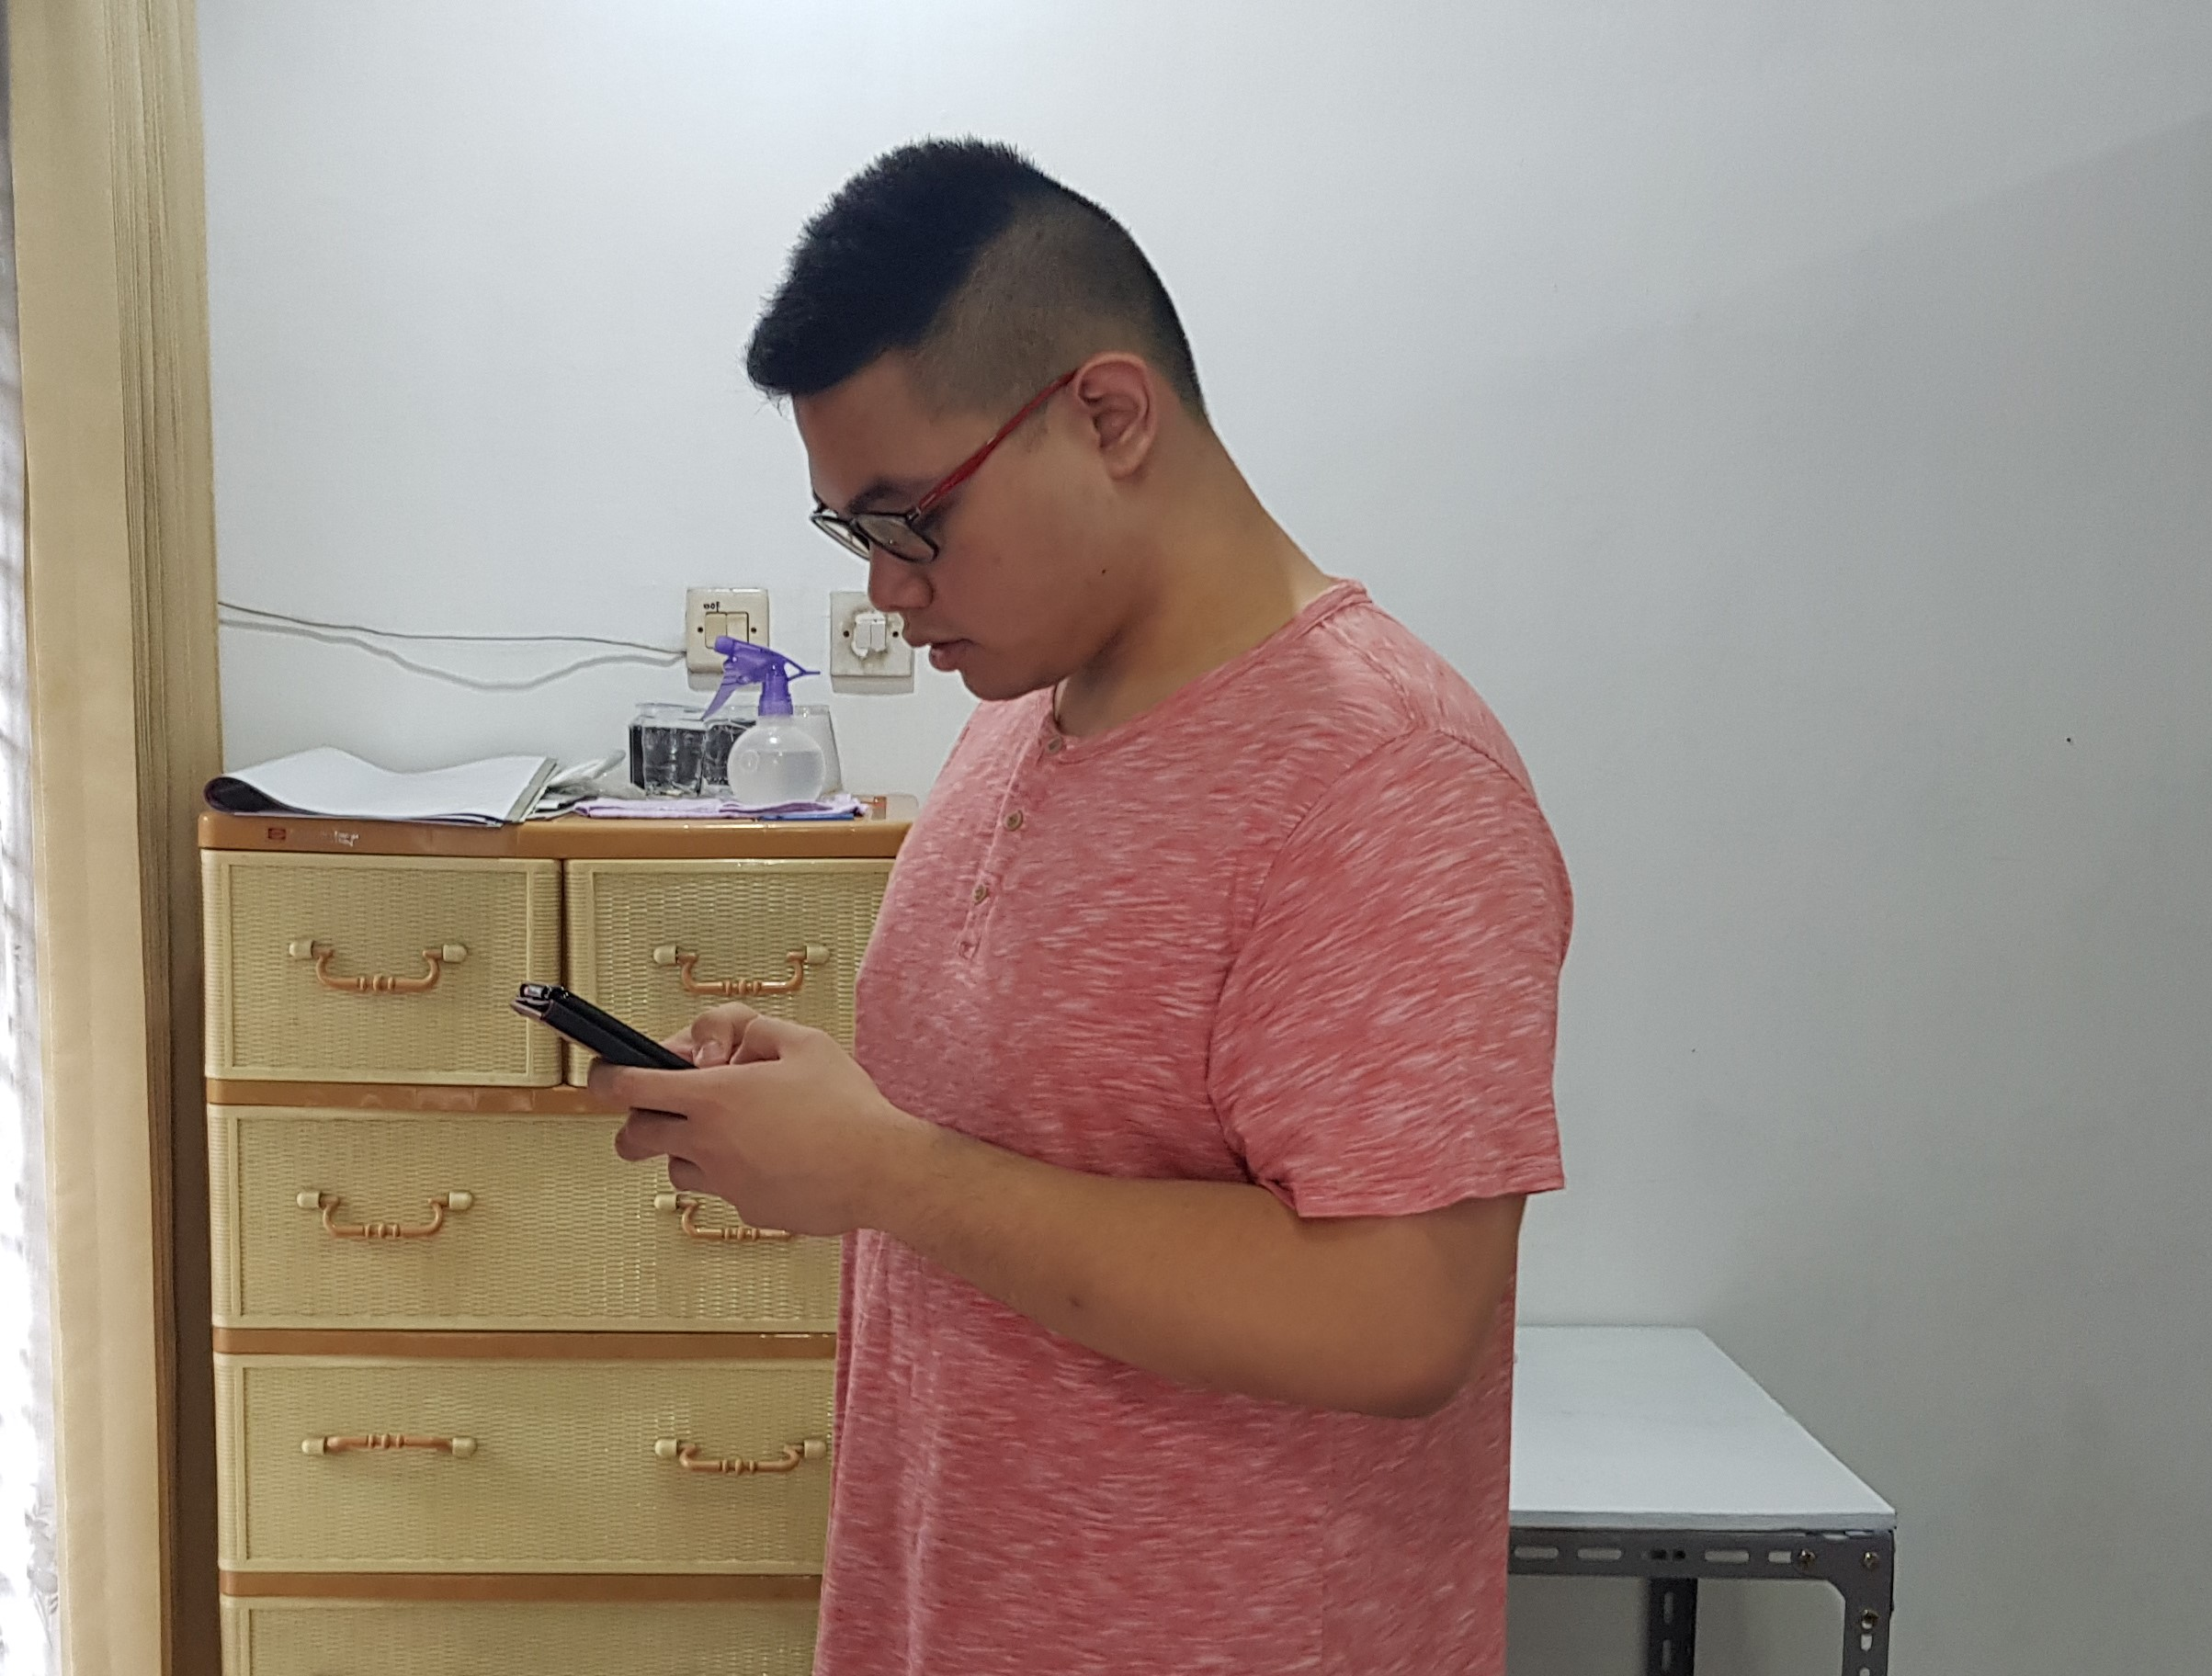
\includegraphics[width=\linewidth]{Gambar/richard-input.jpg}
  \caption{Ilustrasi Pengguna saat Memasukkan Masukan Lokasi Asal dan Tujuan}
  \label{fig:user-main-page}
\endminipage\hfill
\end{figure}


\subsubsection{Tampilan ketika Tombol Ditekan dengan \textit{Textbox} dalam Keadaan Kosong}
Ketika pengguna menekan tombol "\textit{Start Running}" dan keadaan salah satu \textit{textbox} kosong, akan ada \textit{Toast} yang memberikan pesan bahwa \textit{textbox} tidak boleh ada dalam keadaan kosong. Gambar \ref{fig:empty-textbox} menunjukkan tampilah \textit{activity} ini.

\begin{figure}
\centering
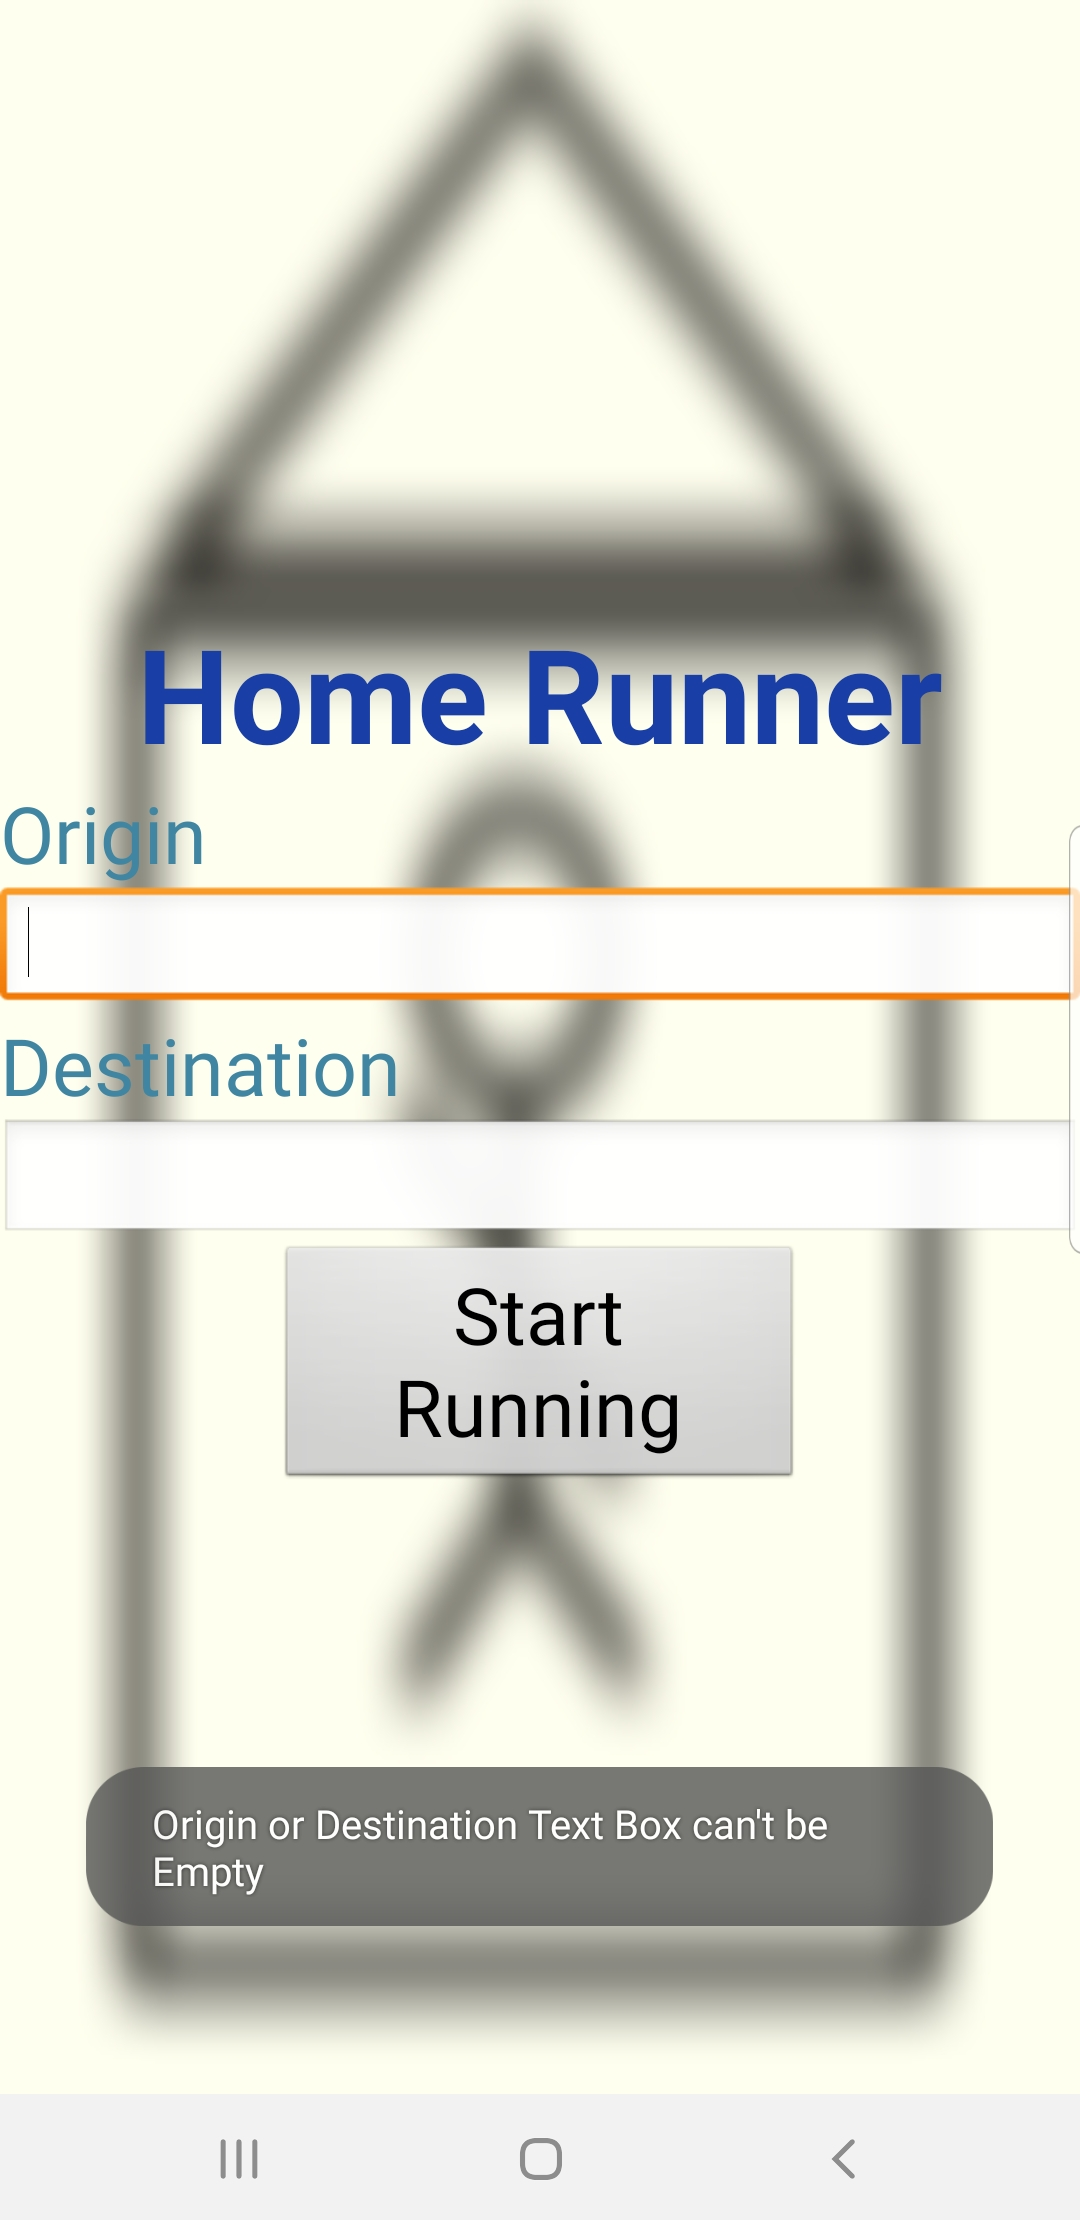
\includegraphics[scale=0.15]{Gambar/empty-textbox.jpg}
    \caption{Tampilan Aplikasi ketika tombol \textit{"Start Running"} Ditekan saat \textit{textbox} \textit{origin} atau \textit{destination} kosong}
    \label{fig:empty-textbox}
\end{figure}


\subsubsection{Aplikasi ketika Masukan Lokasi yang Sah Dimasukkan, Saat Gawai dalam Posisi \textit{Portrait}}
Saat masukan yang sah dimasukkan pengguna, pengguna akan langsung diarahkan ke halaman yang memberitahu untuk mempersiapkan \textit{Cardboard viewer}, memutar gawai agar menjadi \textit{landscape}. Gambar \ref{fig:cardboard-page} menunjukkan tampilan peringatan ini dan Gambar \ref{fig:user-transition-page} mengilustrasikan \textit{state} dari pengguna.

\begin{figure}
\minipage{0.5\textwidth}
  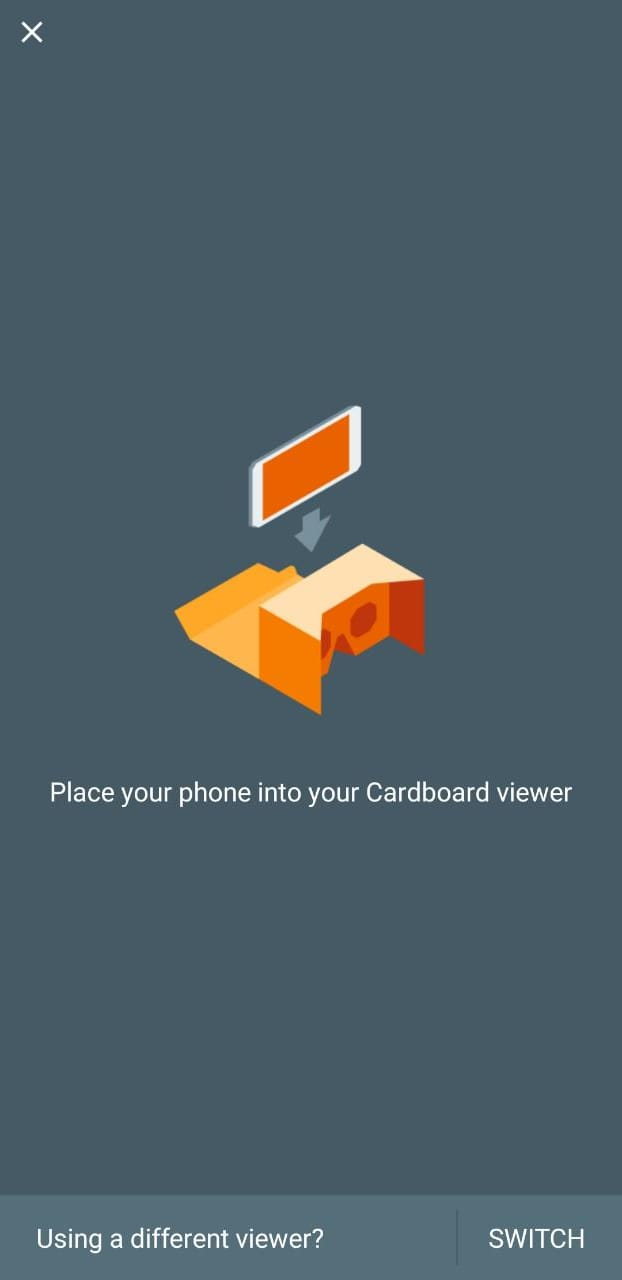
\includegraphics[scale=0.2]{Gambar/cardboard-page.png}
    \caption{Tampilan \textit{Google Cardboard} sebelum gawai diputar}
    \label{fig:cardboard-page}
\endminipage\hfill
\minipage{0.5\textwidth}
  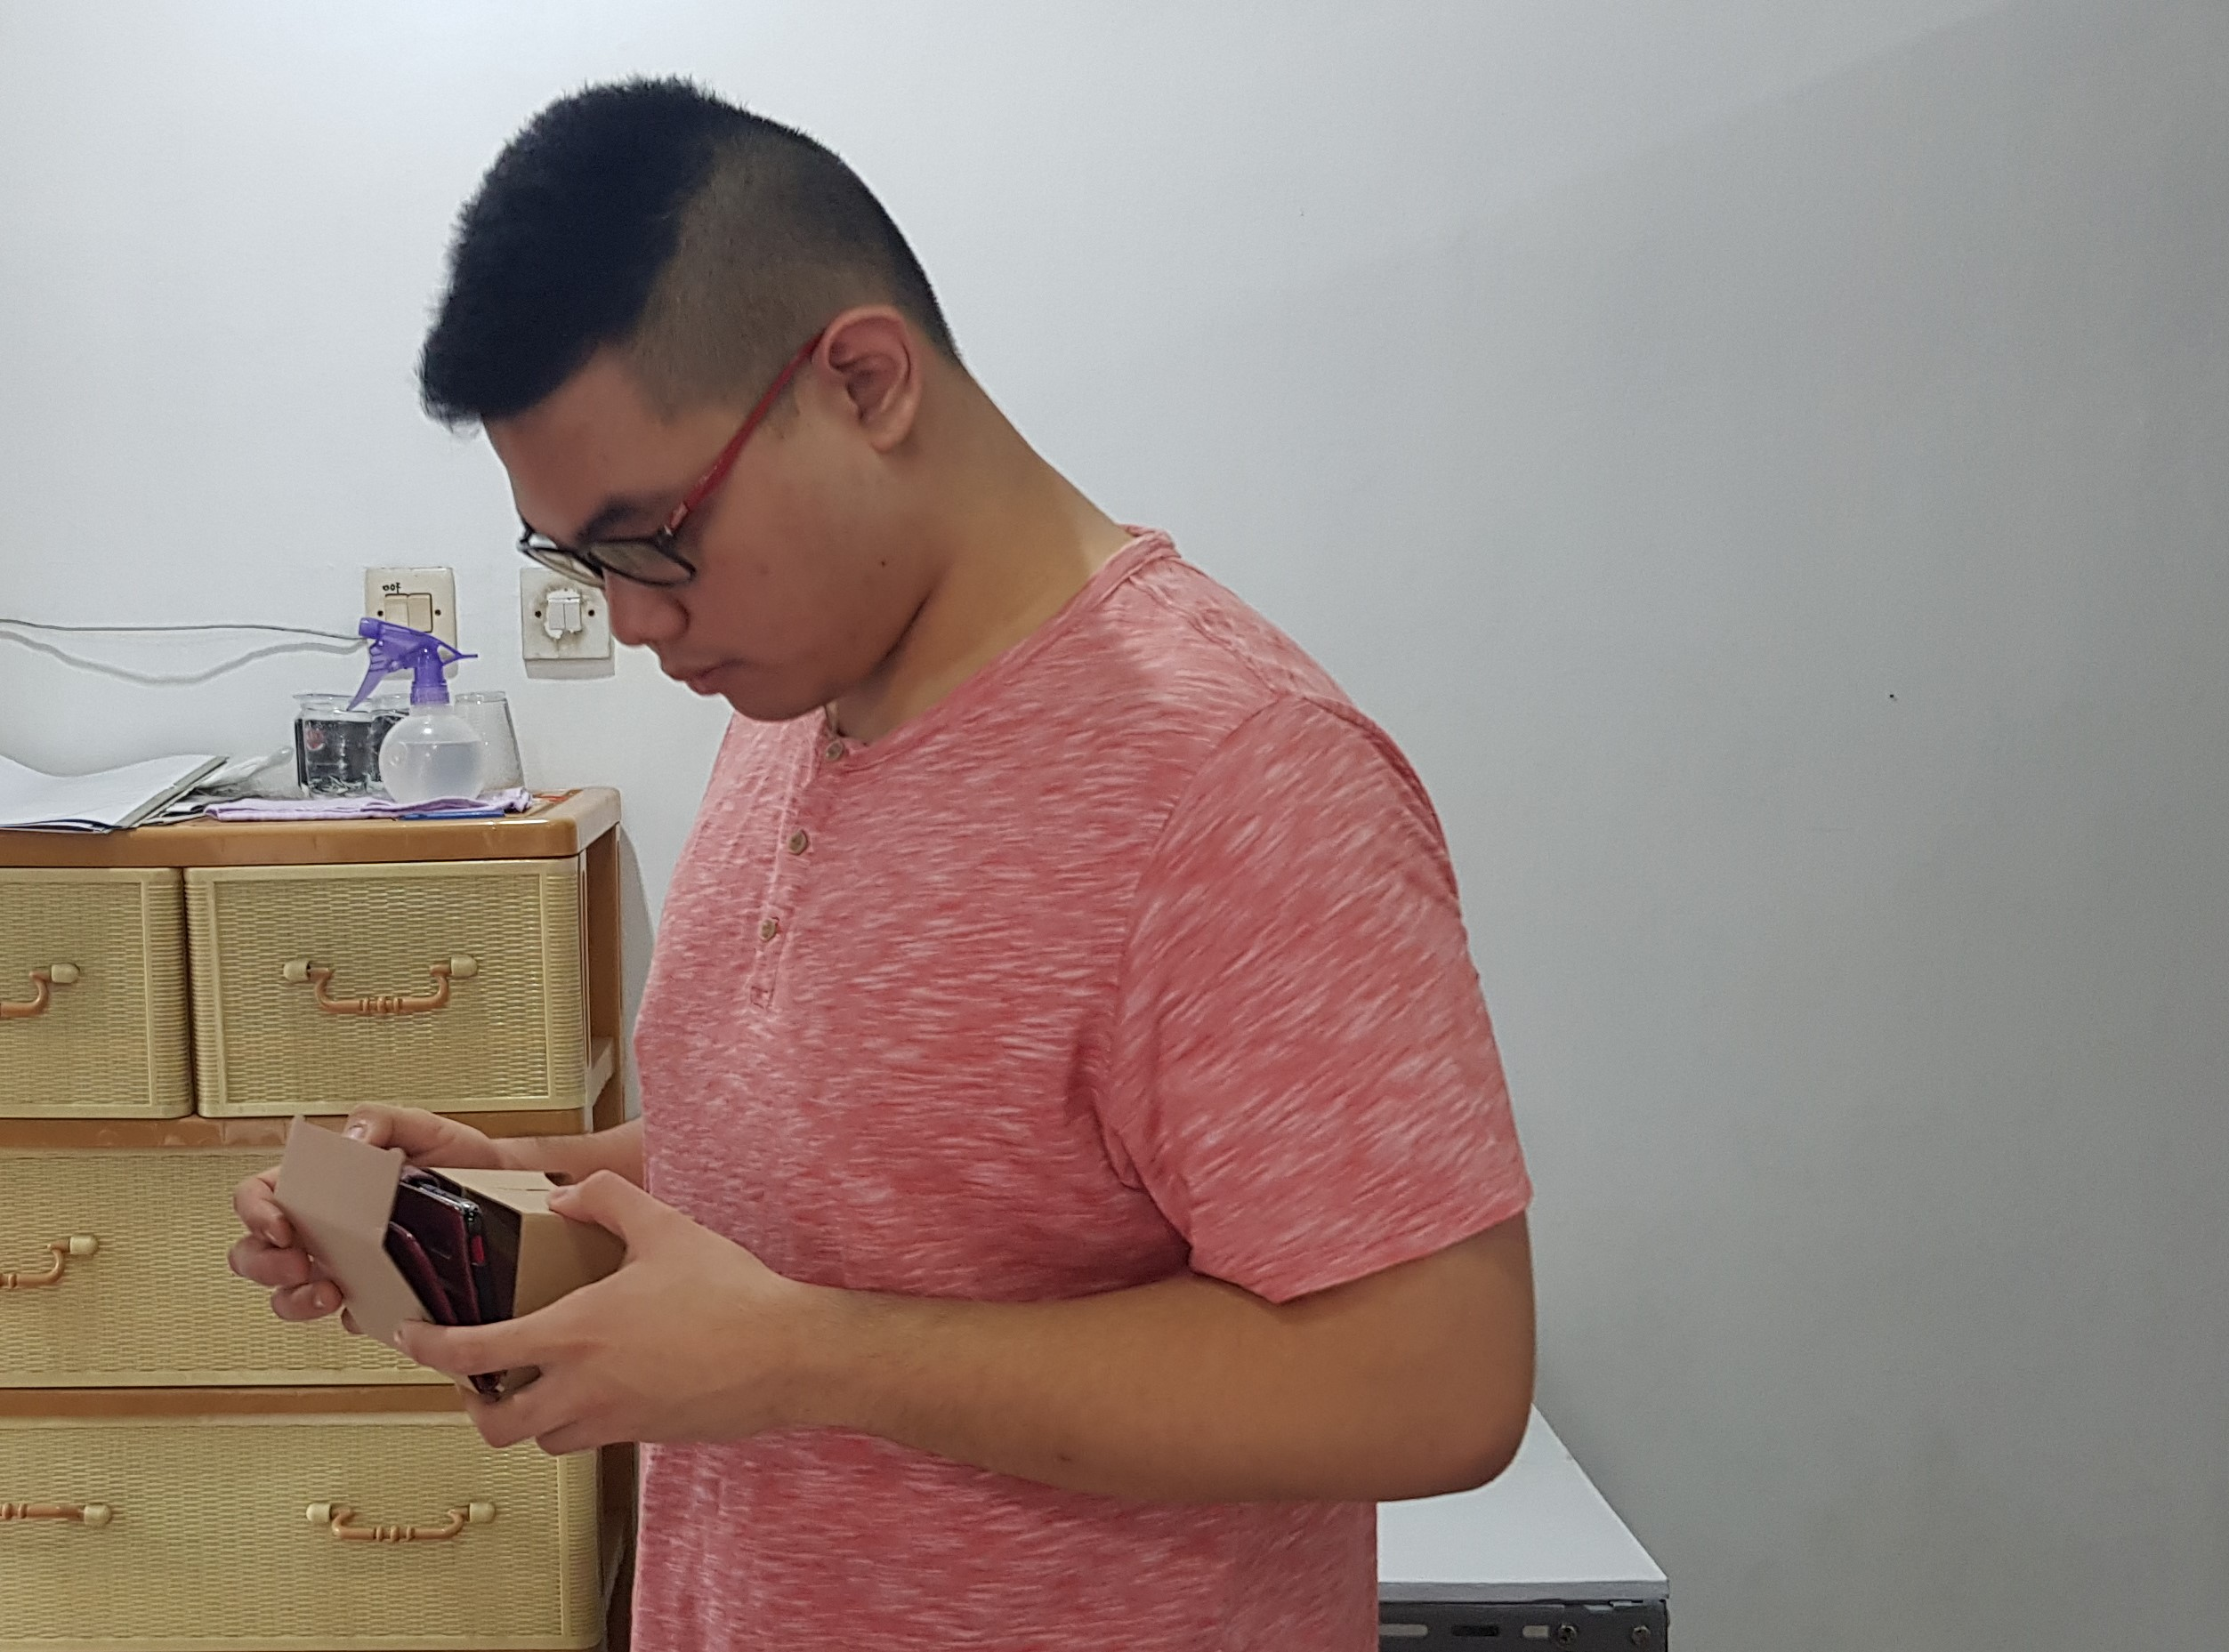
\includegraphics[width=\linewidth]{Gambar/richard-vr-setup.jpg}
  \caption{Ilustrasi Pengguna saat Melihat Tampilan Aplikasi Tersebut}
  \label{fig:user-transition-page}
\endminipage\hfill
\end{figure}

\subsubsection{Aplikasi saat Pengguna Berlari}
Setelah memasukkan masukan lokasi asal dan tujuan yang benar lewat dua \textit{textbox}, siap dengan \textit{Cardboard viewer} dan gawai berada dalam posisi \textit{landscape},  aplikasi akan menampilkan dunia VR dengan pemandangan sesuai dengan lokasi asal, dan pemandangan akan berubah sesuai jarak yang pengguna telah tempuh. \textit{Activity} VR saat pengguna berlari digambarkan pada Gambar \ref{fig:vr-page} dan Gambar \ref{fig:user-vr-page} menunjukkan \textit{state} pengguna.

\begin{figure}
\minipage{0.5\textwidth}
  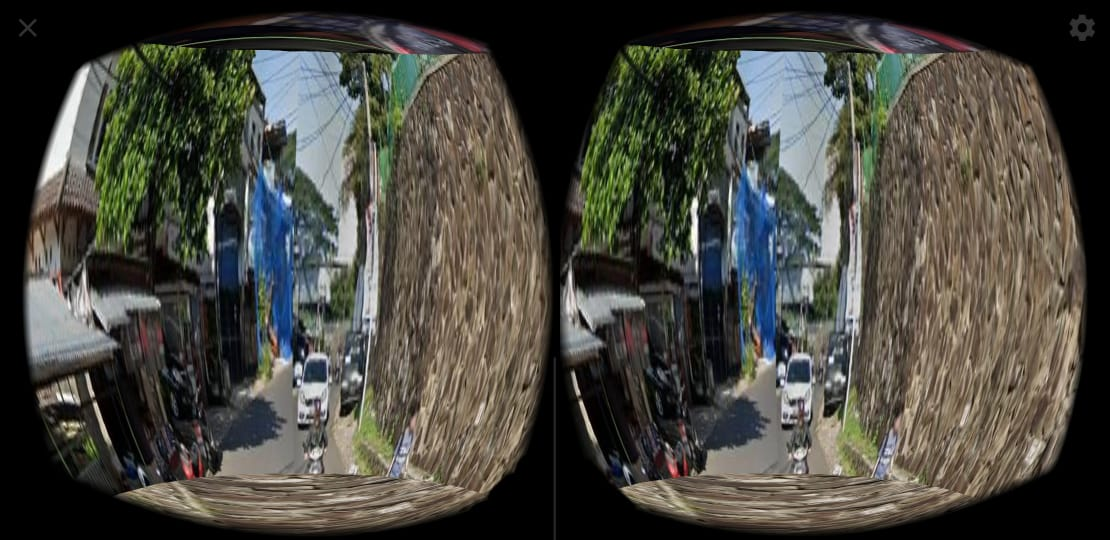
\includegraphics[scale=0.1]{Gambar/vr-page.png}
    \caption{Tampilan VR saat Pengguna Berlari}
    \label{fig:vr-page}
\endminipage\hfill
\minipage{0.5\textwidth}
  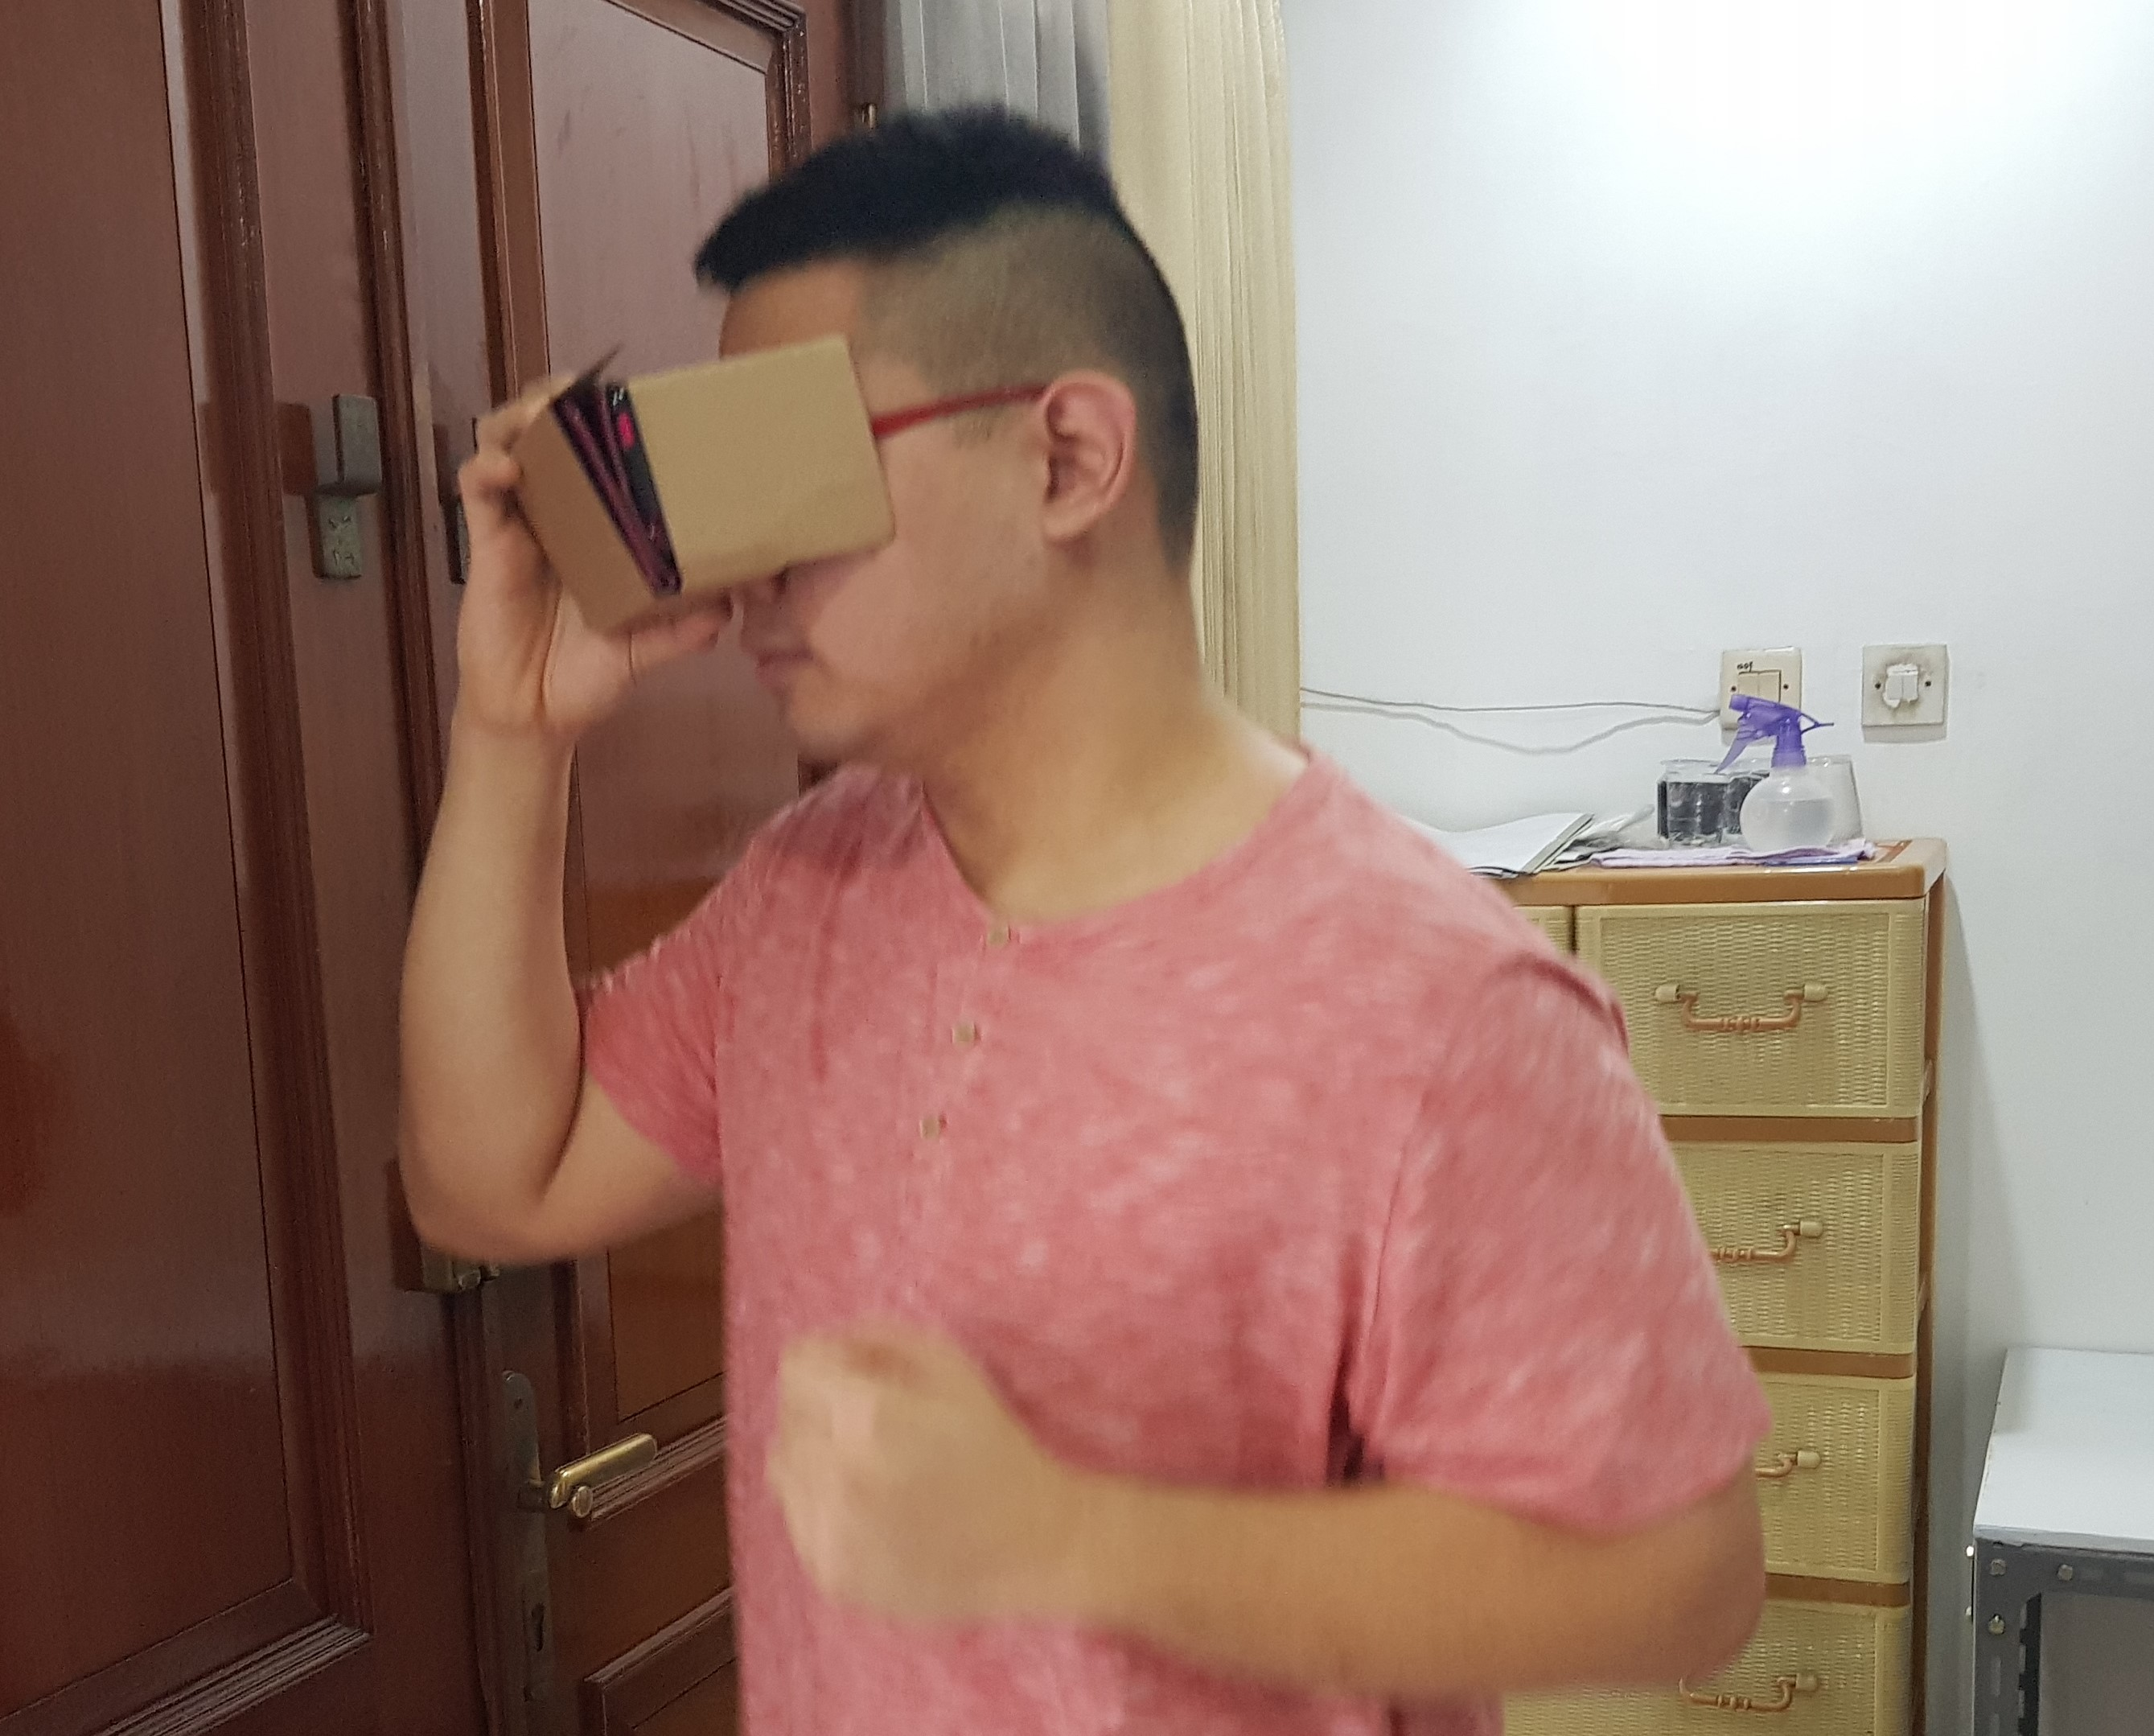
\includegraphics[width=\linewidth]{Gambar/richard-running.jpg}
  \caption{Ilustrasi Pengguna saat Berlari}
  \label{fig:user-vr-page}
\endminipage\hfill
\end{figure}

\subsection{Aplikasi Setelah Pengguna Menyelesaikan Perjalanannya}
Ketika pengguna sudah berlari sampai tujuan, tampilan dengan tulisan "\textit{Congratulations! You finished your run}". Gambar \ref{fig:finished-page} menunjukkan halaman ini.

\begin{figure}
\centering

\includegraphics[scale=0.15]{Gambar/finished-page.png}
    \caption{Tampilan VR saat Pengguna Mencapai Tujuan}
    \label{fig:finished-page}
\end{figure}

\section{Pengujian}
Pengujian dilakukan dalam dua metode: fungsional dan eksperimental. Pengujian fungsional dilakukan untuk menguji apakah aplikasi sudah berfungsi dengan seharusnya, sedangkan pengujian eksperimental ditujukan untuk mengetahui fungsi sensor \textit{step detector} dalam aplikasi pada beberapa perangkat yang digunakan dalam pengujian fungsional.

\subsection{Pengujian Fungsional}
\label{subs:fungtional-test}
Hal pertama yang dilakukan pada pengujian fungsional ini adalah mencoba meng-\textit{install} aplikasi pada tiga perangkat dengan spesifikasi yang dirincikan pada Tabel \ref{tab:hardware-test}. 

\begin{table}[]
    \centering
    \caption{Daftar Perangkat yang digunakan dalam Pengujian}
    \begin{tabular}{|p{1cm}||p{4cm}|p{4cm}|p{3cm}|}
    \hline
       No  & Processor & Sistem Operasi & RAM \\
    \hline
        1 &  Qualcomm Snapdragon 835 2.45 GHz & Android OS v9.0 (Pie) & 6GB\\
    \hline
        2 &  Quad-Core 2.3 GHz & Android v5.0 (Lollipop) & 4GB \\
    \hline
        3 &  1.6GHz octa-core & Android OS v8.1 (Oreo) & 2GB\\
    \hline
    \end{tabular}
    \label{tab:hardware-test}
\end{table}

Setelah memasang aplikasi pada mamsing-masing perangkat, pengujian fungsional dapat dilakukan dengan mempersiapkan himpunan masukan dengan keluaran yang diharapkan, lalu memasukkan setiap masukan pada himpunan masukan pada setiap perangkat saat menjalankan aplikasi. Tabel \ref{tab:input-test} memperlihatkan masukan pengujian beserta hasil yang diharapkan. 

\begin{table}[]
    \centering
    \caption{Himpunan Masukan untuk Pengujian Aplikasi}
    \begin{tabular}{|p{3cm}||p{5cm}|p{7cm}|}
    \hline
       Nomor Masukan & Masukan \textit{origin},\textit{destination}  & Hasil yang Diharapkan\\
    \hline  \hline
     1 & "unpar","bip,bandung"   & Berhasil menampilkan pemandangan di sekitar Universitas Katolik Parahyangan, dapat berjalan sampai Bandung Indah Plaza, lalu menampilkan tulisan "Congratulations"\\ \hline
     2 & "unpar","bandung indah plaza" & 
     Berhasil menampilkan pemandangan di sekitar Universitas Katolik Parahyangan, dapat berjalan sampai Bandung Indah Plaza, lalu menampilkan tulisan "Congratulations"\\ 
     \hline
     3 & "universitas katolik parahyangan","bip,bandung" & Berhasil menampilkan pemandangan di sekitar Universitas Katolik Parahyangan, dapat berjalan sampai Bandung Indah Plaza, lalu menampilkan tulisan "Congratulations"\\    \hline
     4 & "universitas katolik parahyangan","bandung indah plaza" & Berhasil menampilkan pemandangan di sekitar Universitas Katolik Parahyangan, dapat berjalan sampai Bandung Indah Plaza, lalu menampilkan tulisan "Congratulations"\\ \hline
     5 & "rs borromeus","rs immanuel" & Berhasil menampilkan pemandangan di sekitar Rumah Sakit Santo Borromeus, dapat berjalan sampai Rumah Sakit Immanuel, lalu menampilkan tulisan "Congratulations"\\ \hline
     6 & "rs boromeus","rs imanuel" & Berhasil menampilkan pemandangan di sekitar Rumah Sakit Santo Borromeus, dapat berjalan sampai Rumah Sakit Immanuel, lalu menampilkan tulisan "Congratulations" \\ \hline
     7 & "ciwalk","boromeus" & Berhasil menampilkan pemandangan di sekitar \textit{Cihampelas Walk}, dapat berjalan sampai Rumah Sakit Santo Borromeus, lalu menampilkan tulisan "Congratulations" \\
     \hline
    \end{tabular}
    \label{tab:input-test}
\end{table}

Masukan 1 sampai 4 ditujukan untuk menguji \textit{string} lokasi yang dieja dengan lengkap dan disingkat pada masing-masing masukan \textit{origin} dan \textit{destionation}. Masukan 5 dan 6 ditujukan untuk menguji masukan dari nama-nama tempat yang umum didengar dan dibicarakan orang, namun jarang ditulis orang sehingga penulisan nama sering kali salah (kekurangan satu huruf dalam pengejaannya).

Setelah himpunan masukan untuk pengujian telah ditentukan, pengujian dilakukan pada masing-masing perangkat. Tabel \ref{tab:test-hardware-one} memperlihatkan hasil pengujian pada Perangkat 1, Tabel \ref{tab:test-hardware-two} memperlihatkan pengujian pada Perangkat 2, Tabel \ref{tab:test-hardware-three} memperlihatkan pengujian pada Perangkat 3.

\begin{table}[]
    \centering
    \caption{Hasil Pengujian pada Perangkat 1}
    \begin{tabular}{|p{3cm}||p{7cm}|p{4cm}|}
    \hline
       Nomor Masukan & Hasil & Status \\
    \hline \hline
        1 & Berhasil menampilkan pemandangan di sekitar Universitas Katolik Parahyangan, dapat berjalan sampai Bandung Indah Plaza, lalu menampilkan tulisan "Congratulations" & Berhasil\\
    \hline
        2 & Berhasil menampilkan pemandangan di sekitar Universitas Katolik Parahyangan, dapat berjalan sampai Bandung Indah Plaza, lalu menampilkan tulisan "Congratulations" & Berhasil \\
    \hline
        3 & Berhasil menampilkan pemandangan di sekitar Universitas Katolik Parahyangan, secara virtual dapat berjalan sampai Bandung Indah Plaza, lalu menampilkan tulisan "Congratulations" & Berhasil \\
        \hline
        4 & Berhasil menampilkan pemandangan di sekitar Universitas Katolik Parahyangan, dapat berjalan sampai Bandung Indah Plaza, lalu menampilkan tulisan "Congratulations" & Berhasil \\
        \hline
        5 & Berhasil menampilkan pemandangan di sekitar Rumah Sakit Boromeus, dapat berjalan sampai Bandung Indah Plaza, lalu menampilkan tulisan "Congratulations" & Berhasil\\ 
        \hline
        6 & Berhasil menampilkan pemandangan di sekitar Rumah Sakit Santo Borromeus, dapat berjalan sampai Rumah Sakit Immanuel, lalu menampilkan tulisan "Congratulations" & Berhasil \\
        \hline 
        7 & Berhasil menampilkan pemandangan di sekitar \textit{Cihampelas Walk}, dapat berjalan sampai Rumah Sakit Santo Borromeus, lalu menampilkan tulisan "Congratulations" & Berhasil \\
    \hline
    \end{tabular}
    \label{tab:test-hardware-one}
\end{table} 

\begin{table}[]
    \centering
    \caption{Hasil Pengujian pada Perangkat 2}
    \begin{tabular}{|p{3cm}||p{4cm}|p{4cm}|}
    \hline
       Nomor Masukan & Hasil & Status \\
    \hline \hline
        1 & Berhasil menampilkan pemandangan di sekitar Universitas Katolik Parahyangan, dapat berjalan sampai Bandung Indah Plaza, lalu menampilkan tulisan "Congratulations" & Berhasil\\
    \hline
        2 & Aplikasi terhenti tiba-tiba & Gagal \\
    \hline
        3 & Aplikasi terhenti secara tiba-tiba & Gagal \\
        \hline
        4 & Aplikasi terhenti secara tiba-tiba & Gagal \\
        \hline
        5 & Aplikasi terhenti tiba-tiba & Gagal \\
        \hline
        6 & Aplikasi terhenti tiba-tiba & Gagal \\
        \hline 
        7 & Berhasil menampilkan pemandangan di sekitar \textit{Cihampelas Walk}, dapat berjalan sampai Rumah Sakit Santo Borromeus, lalu menampilkan tulisan "Congratulations" & Berhasil\\
        \hline
    \end{tabular}
    \label{tab:test-hardware-two}
\end{table} 

\begin{table}[]
    \centering
    \caption{Hasil Pengujian pada Perangkat 3}
    \begin{tabular}{|p{3cm}||p{4cm}|p{4cm}|}
    \hline
       Nomor Masukan & Hasil & Status \\
    \hline \hline
        1 & Aplikasi menampilkan lokasi asal, namun gambar berhenti & Gagal\\
    \hline
        2 & Aplikasi menampilkan lokasi asal, namun gambar berhenti & Gagal \\
    \hline
        3 & Aplikasi menampilkan lokasi asal, namun gambar berhenti & Gagal \\
        \hline
        4 & Aplikasi menampilkan lokasi asal, namun gambar berhenti & Gagal \\
        \hline
        5 & Aplikasi menampilkan lokasi asal, namun gambar berhenti & Gagal \\
        \hline
        6 & Aplikasi menampilkan lokasi asal, namun gambar berhenti & Gagal \\
        \hline
        7 & Aplikasi menampilkan lokasi asal, namun gambar berhenti & Gagal \\ 
        \hline
    \end{tabular}
    \label{tab:test-hardware-three}
\end{table}

Pada Perangkat 1, aplikasi berjalan dengan sangat lancar, mengeluarkan hasil yang sesuai dengan yang diharapkan pada semua masukan.

Pada Perangkat 2, aplikasi hanya berhasil pada Masukan 1 dan 7, tetapi masukan-masukan yang lain membuat aplikasi terhenti secara tiba-tiba, yaitu masukan yang memiliki karakter spasi (\textit{whitespace)}. Hal ini mungkin disebabkan \textit{operating system} (OS) yang kurang tinggi sehingga \textit{character coding} pada \textit{textbox} masukan tidak dapat dilakukan dengan baik sehingga mengolah \textit{string URL} menjadi sesuatu hal yang tidak dapat diproses aplikasi. 

Pada Perangkat 3, aplikasi tidak dapat berfungsi dengan baik karena pada tampilan VR, aplikasi tidak dapat merespon terhadap pergerakan yang terjadi pada perangkat. Pemandangan VR langsung terhenti dan tidak bisa berlanjut sampai berlari ke tujuan. Hal ini diduga karena ukuran RAM yang kurang sehingga tidak dapat menjalankan aplikasi dengan seharusnya.

\subsection{Pengujian Eksperimental}
Pada pengujian eksperimental, akan dilakukan \textit{logging} untuk melihat jarak yang ditempuh pada \textit{virtual jogging app}. Perangkat yang digunakan untuk pengujian ini adalah Perangkat 1 dan 2 yang dijelaskan pada Subbab \ref{subs:fungtional-test}. Perangkat 3 tidak digunakan karena aplikasi tidak dapat berjalan dengan seharusnya pada perangkat ini. Masukan untuk aplikasi pada masing-masing aplikasi adalah "unpar" untuk lokasi asal dan "bip,bandung" untuk lokasi tujuannya.

Gambar \ref{fig:samsung-note-8-exp} dan Gambar \ref{fig:asus-zenfone-2-exp} menampilkan \textit{logging} dari beberapa langkah terakhir perjalanan. 

\begin{figure}[h]
	\centering	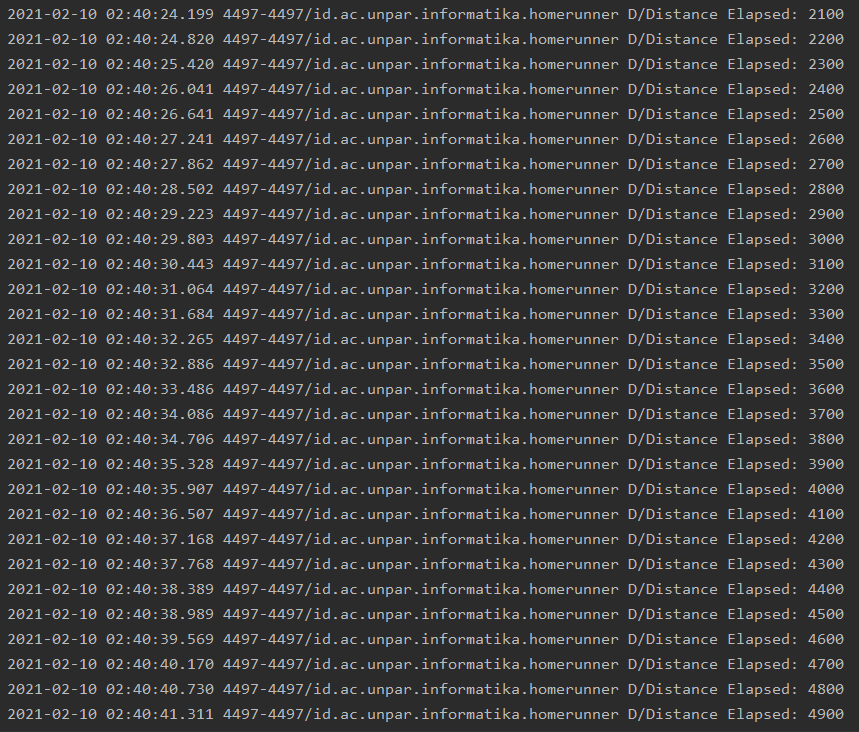
\includegraphics[scale=1]
	{Gambar/samsung-note-8-exp.png}
	\caption{\textit{Log console} yang Menampilkan Jarak Tempuh Pengguna pada Perangkat 1}
	\label{fig:samsung-note-8-exp}
\end{figure}

\begin{figure}[h]
	\centering	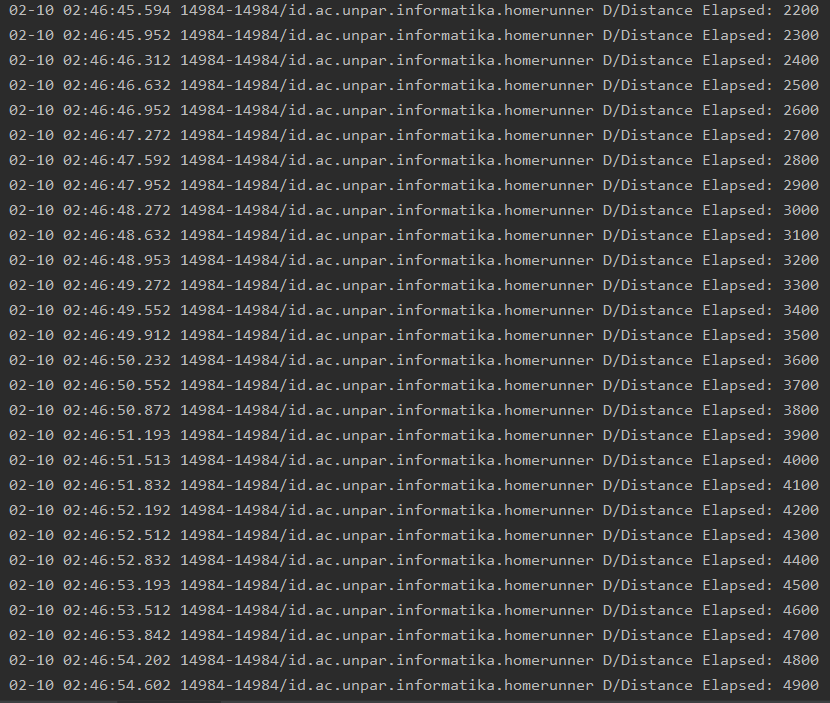
\includegraphics[scale=1]
	{Gambar/asus-zenfone-2-exp.png}
	\caption{\textit{Log console} yang Menampilkan Jarak Tempuh Pengguna pada Perangkat 2}
	\label{fig:asus-zenfone-2-exp}
\end{figure}

Dari \textit{log console virtual jogging app}, dapat dilihat bahwa pada masing-masing perangkat, jarak tempuh pengguna terlihat bertambah setiap menerima rangsang yang adalah langkah  kaki pengguna. Hasil yang ditampilkan pada masing-masing \textit{log console} serupa. 


\section{Masalah yang Dihadapi}
Adapun masalah-masalah yang dihadapi dalam proses pengembangan aplikasi adalah sebagai berikut:

\begin{enumerate}
	\item Munculnya galat pada saat mencoba menggambar ulang bangun ruang silinder dengan tekstur baru. Galat tersebut adalah pemanggilan \textit{OpenGL renderer} pada \textit{thread} yang tidak memiliki \textit{context}. Rencana awalnya adalah melakukan \textit{load StreetView API} dari pemandangan selanjutnya pada saat sensor \textit{step detector} mendeteksi langkah kaki, lalu mengubah tekstur bangun ruang silinder. 
	
	\item Peng-\textit{update}-an \textit{Gradle} di Android Studio membuat terjadinya \textit{compile error} sehingga diperlukan waktu untuk memperbaiki galat ini dan menghambat perkembangan aplikasi. 
\end{enumerate}

